% JointGuard AI - technical report.
% Compile with pdfLaTeX (e.g. on Overleaf): upload this file together with the figures/ folder.
% All numbers come from results/standard/*.json and models/standard/*.json (seed 20261024).
\documentclass[11pt,a4paper]{article}
\usepackage[margin=2.4cm]{geometry}
\usepackage[T1]{fontenc}
\usepackage{lmodern}
\usepackage{amsmath,amssymb}
\usepackage{siunitx}
\usepackage{graphicx}
\usepackage{booktabs}
\usepackage{tabularx}
\usepackage{caption}
\usepackage{enumitem}
\usepackage{xcolor}
\usepackage[colorlinks=true,linkcolor=blue!50!black,urlcolor=blue!50!black,citecolor=blue!50!black]{hyperref}
\setlist{itemsep=2pt,topsep=4pt}
\graphicspath{{figures/}}

% ---------------------------------------------------------------- links
% Fill these in before compiling. Leave a link as \missinglink if you do not have it yet.
\newcommand{\missinglink}{\textcolor{red!70!black}{[link to be added]}}
\newcommand{\linkcode}{\url{https://github.com/chechoutanh/JointGuard-AI}}
\newcommand{\linkpage}{\missinglink}      % project web page (shared link)
\newcommand{\linkreportvi}{\href{https://github.com/chechoutanh/JointGuard-AI/blob/main/reports/standard/report_en.md}{\texttt{reports/standard/report\_en.md} on GitHub}}

\title{\textbf{JointGuard AI}\\[4pt]
\large Detecting and Diagnosing Abnormal Joint Friction in a Simulated Robot Arm}
\author{Tuan Anh Nguyen}
\date{October 2026}

\begin{document}
\maketitle

\begin{abstract}
\noindent
Rising friction in a robot joint is an early sign of mechanical trouble, but the signals it changes, joint torque and
tracking error, also change when a healthy arm carries a heavier load or moves faster. This project asks whether a
model that sees only those two signals can raise an alarm for abnormal friction without raising one for these
harmless changes, and whether it can then say which joint is affected and by how much. I built a physics-based
simulator of a two-joint arm, injected friction faults in a controlled way, and trained Random Forest models on
causal window features. Inside the range of conditions seen in training, the detector caught 32 of 32 faulty test
runs with a median delay of 1.5\,s and 0.21 false alarms per minute, against 16 of 32 for an error-threshold
baseline. A diagnosis stage named the correct joint in 30 of 32 detected runs, with a median error of 0.36 in the
estimated friction multiplier. On a held-out stress test with heavier loads, faster motion and an unseen trajectory
type, false alarms rose to 3.88 per minute, so the model does not generalise beyond its training range. All data is
simulated and nothing has been validated on a physical robot.
\end{abstract}

\section{Motivation and research question}
During a summer internship in a university control and automation lab, I worked with industrial robot arms and their
control software. Maintenance on such arms is usually scheduled or reactive. A system that notices a joint becoming
harder to move, from signals the controller already has, could flag problems earlier without adding sensors.

The difficulty is that higher friction is not the only thing that raises torque and tracking error. A healthy arm
that carries more weight needs more torque, and a healthy arm that moves faster lags further behind its target. A
detector that reacts to any increase would raise false alarms in normal operation. The research question is therefore:

\begin{quote}
\emph{Using only joint torque and tracking error, can a model detect that one joint's friction has risen abnormally,
without false alarms when a healthy arm carries a heavier load or moves faster? Once it raises an alarm, can it
identify the joint and estimate how much its friction has risen?}
\end{quote}

\noindent
The problem has three separate parts: \emph{detect} (is something abnormal?), \emph{diagnose} (which joint, how
much?) and \emph{estimate wear} (how long until failure?). Each needs different evidence. This report covers the
first two. Estimating wear needs run-to-failure data recorded over a component's life, which a simulation of
injected faults cannot provide.

\section{Simulation}
\subsection{Arm dynamics}
The arm has two revolute joints and moves in a vertical plane, so gravity acts on it. Its motion follows
\begin{equation}
  M(q)\,\ddot q + C(q,\dot q)\,\dot q + G(q) + \tau_f(\dot q) = \tau_{\text{applied}},
  \label{eq:dyn}
\end{equation}
where $q=(q_1,q_2)$ are the joint angles ($q_2$ relative to link 1), $M$ is the inertia matrix, $C\dot q$ holds
Coriolis and centrifugal terms, $G$ is gravity and $\tau_f$ is joint friction. At each step the simulator solves the
$2\times2$ linear system for $\ddot q$ and integrates the state with a fourth-order Runge--Kutta method at
\SI{1}{ms}. A payload at the tip is modelled as a point mass merged into link 2, so it changes both $M$ and $G$
consistently. The arm's motion is never copied from the target path; it only comes from integrating
\eqref{eq:dyn}.

\begin{table}[h]
\centering
\caption{Arm and controller parameters (SI units).}
\begin{tabular}{lrr}
\toprule
Parameter & Link 1 & Link 2 \\
\midrule
Length [m] & 0.60 & 0.50 \\
Mass [kg] & 8.0 & 5.0 \\
Inertia about centre of mass [kg\,m$^2$] & 0.24 & 0.104 \\
Rotor inertia (reflected) [kg\,m$^2$] & 0.15 & 0.08 \\
Torque limit [N\,m] & 150 & 60 \\
Nominal viscous friction $b$ [N\,m\,s/rad] & 2.0 & 1.2 \\
Nominal Coulomb friction $\tau_c$ [N\,m] & 3.0 & 2.0 \\
Controller gains $K_p$ / $K_d$ & 1500 / 100 & 300 / 20 \\
\bottomrule
\end{tabular}
\end{table}

Physics checks run as automated tests: forward kinematics at known poses, symmetry and positive definiteness of $M$,
$G$ equal to the gradient of potential energy, energy conservation without friction or torque, energy loss with
friction, and absence of numerical blow-up. Halving the time step to \SI{0.5}{ms} in a run with a $\times4$ fault and
a \SI{2}{kg} payload changed joint angles by at most $8.2\times10^{-9}$\,rad.

\subsection{Controller and sensors}
A PD controller with gravity compensation runs at \SI{100}{Hz} on noisy measurements,
\begin{equation}
  \tau_{\text{req}} = K_p\,(q_{\text{des}} - q_{\text{meas}}) + K_d\,(\dot q_{\text{des}} - \dot q_{\text{meas}})
  + \hat G(q_{\text{meas}}),
\end{equation}
followed by torque saturation. The controller knows the nominal arm and the declared payload (which may differ from
the real one by up to \SI{0.1}{kg}), but it does \emph{not} know or compensate friction. Higher friction therefore
appears as larger tracking error and larger PD torque. Gaussian noise is added to measured angles and velocities,
with a standard deviation drawn per run from the same range for healthy and faulty runs.

\subsection{Friction and fault model}
Friction at each joint has a viscous and a smoothed Coulomb part. A fault multiplies both by a factor $m\geq1$:
\begin{equation}
  \tau_f = m\left(b\,\dot q + \tau_c \tanh\!\left(\frac{\dot q}{0.02}\right)\right).
\end{equation}
Healthy friction varies by $\pm15\%$ between runs. A window is labelled \emph{anomalous} when $m\geq1.5$ for one
joint; this definition was fixed before any data was generated and does not use tracking error. Faults come in three
shapes: \emph{mild} jumps ($m\in[1.6,2.2]$), \emph{severe} jumps ($m\in[2.8,4.0]$), and \emph{gradual} ramps from 1 to
$[2.2,4.0]$ over 6--12\,s. Only one joint is faulty at a time. Increased friction is one way of modelling a fault; it
does not identify a physical cause such as lost lubrication.

\section{Data and evaluation protocol}
The dataset contains 300 runs of 25\,s, sampled at \SI{100}{Hz}, with no numerical failures. In-range runs use
sinusoidal joint trajectories with frequencies of 0.15--0.55\,Hz. Healthy runs vary speed (payload 0.3--0.8\,kg) or
payload (0--2\,kg). A separate \emph{stress} set, never used for training or tuning, uses heavier payloads (2--3\,kg),
faster motion (0.55--0.75\,Hz) and, in half of its runs, a point-to-point trajectory type not seen in training.

\begin{table}[h]
\centering
\caption{Runs per scenario and split.}
\begin{tabular}{lrrrr}
\toprule
Scenario & Train & Val & Test & Stress \\
\midrule
healthy (speed varied) & 24 & 8 & 8 & 10 \\
healthy (payload varied) & 24 & 8 & 8 & 10 \\
mild, joint 1 / joint 2 & 16 / 16 & 6 / 6 & 6 / 6 & 6 / 6 \\
severe, joint 1 / joint 2 & 16 / 16 & 4 / 4 & 4 / 4 & 6 / 6 \\
gradual, joint 1 / joint 2 & 16 / 16 & 6 / 6 & 6 / 6 & 8 / 8 \\
\bottomrule
\end{tabular}
\end{table}

\noindent Several design choices protect the results from optimistic bias:
\begin{itemize}
  \item Runs come in groups that share a trajectory, payload and healthy friction. Splitting is done by group (60/20/20),
        so near-duplicate runs never appear on both sides of a split. The split file is written before training.
  \item Every choice of features, hyper-parameters, thresholds and alarm rules uses training and validation data only.
  \item Test and stress results are reported separately and never averaged.
  \item Ground truth (true payload, friction multiplier, labels) is stored apart from the observed signals and is never
        a model input. Automated tests check this, check that features are causal, and check that the online and
        offline feature code produce identical numbers.
\end{itemize}

\noindent An \emph{alarm event} is one off-to-on transition. A \emph{false alarm} is an alarm that starts before the
fault is injected; rates are given per minute of healthy operation. \emph{Delay} is measured from the moment the label
switches to anomalous. An alarm that was already on before the fault is never counted as a detection.

\section{Detection}
\subsection{Features}
Every 0.1\,s the detector summarises the last 1.0\,s of samples (window length chosen on validation from 0.5 and 1.0\,s)
into 12 features per joint: torque RMS, standard deviation and peak; RMS rate of change of torque; mean torque along
the direction of target motion; RMS and peak position error; mean position error along the direction of motion; RMS
velocity error; RMS target speed and acceleration; and mean target angle. The direction-weighted error,
\begin{equation}
  \bar e_{\text{dir}} = \frac{1}{N}\sum_{k=1}^{N} e_k \tanh\!\left(\frac{\dot q_{\text{des},k}}{0.05}\right),
\end{equation}
is the key idea. Friction always opposes motion, so it makes the arm lag behind its target \emph{in the direction it
is moving}. Extra payload mainly adds a gravity load, which the controller already compensates. The target-motion
features give the model context, so that a large error caused by fast motion is not mistaken for friction.

Figure~\ref{fig:signature} shows this on recorded demonstration runs. A heavier payload shifts windows to the right
(more torque), while tripled friction shifts them upward (more lag along the motion). The separation is clear for
joint 2 and partial for joint 1, which carries much larger torques.

\begin{figure}[h]
\centering
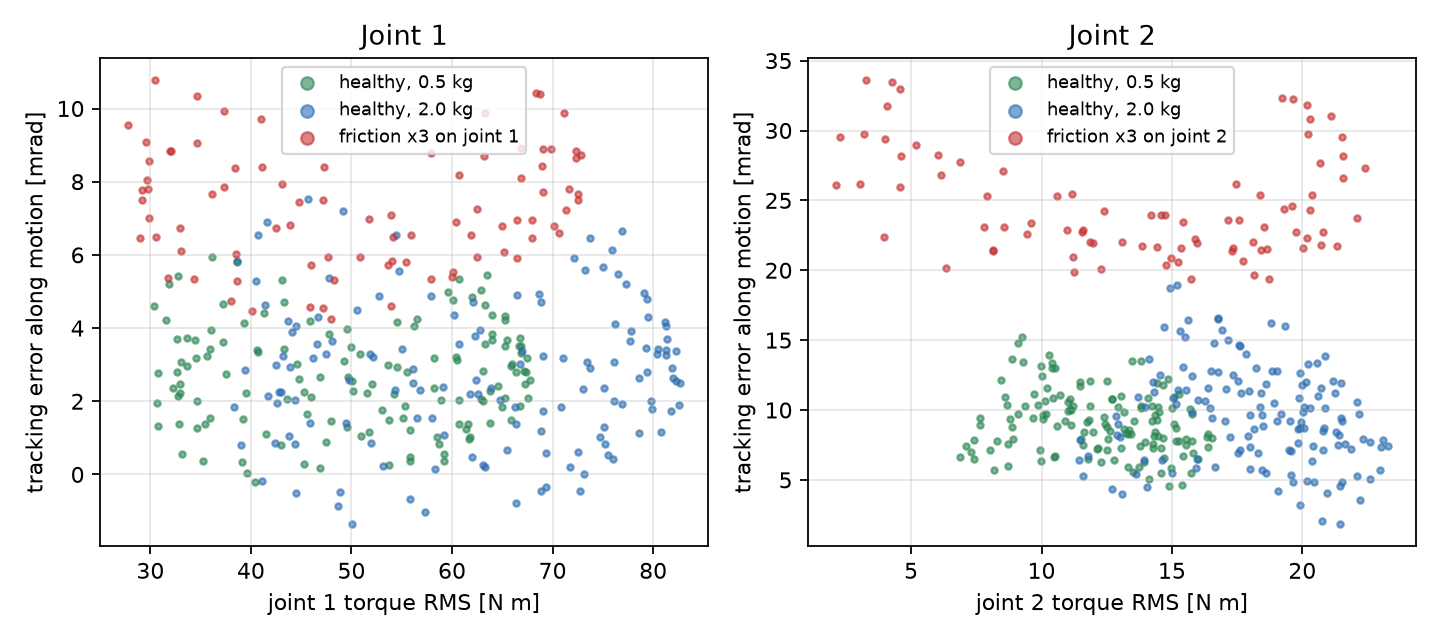
\includegraphics[width=\linewidth]{signature_load_vs_friction.png}
\caption{Torque RMS against direction-weighted tracking error for 1\,s windows from three recorded runs.
Friction windows are taken from 1\,s after the fault.}
\label{fig:signature}
\end{figure}

\subsection{Model and alarm rule}
A Random Forest with 200 trees (minimum 2 samples per leaf, $\sqrt{d}$ features per split) was selected from 32
configurations by validation average precision (0.927). Windows whose label changes inside them were excluded from
training. The forest's output is used as a score, not a calibrated probability. An alarm turns on after
8 consecutive windows score at least 0.40 and turns off after 5 consecutive windows below it. The threshold and the
value 8 were chosen on validation to maximise F1 subject to at most 0.5 false alarms per minute. The chosen value 8 lies
at the edge of the search grid $\{1,3,5,8\}$; this is reported rather than adjusted after seeing test results.

The \emph{baseline} scores a window by $\max_j \text{RMS}(e_j)/r_j$, where $r_j$ is the 95th percentile of healthy
training windows, and uses the same alarm logic and the same validation procedure.

The most important features (impurity-based) are all tracking-error features: joint 1 error along the motion (13.8\%),
joint 2 error RMS (10.1\%) and joint 2 error along the motion (9.3\%).

\subsection{Results}
\begin{table}[h]
\centering
\caption{Detection results. FA/min: false alarms per minute of healthy operation. Healthy w/ FA: healthy runs with at
least one false alarm. F1 compares the alarm state with the label on every window, including the delay period.}
\label{tab:det}
\small
\begin{tabular}{llrrrrr}
\toprule
Set & Detector & Detected & FA/min & Healthy w/ FA & Median delay [s] & F1 \\
\midrule
Test & Random Forest & 32/32 & 0.21 & 0/16 & 1.5 & 0.82 \\
     & Baseline      & 16/32 & 0.31 & 0/16 & 2.7 & 0.43 \\
\midrule
Stress & Random Forest & 26/40 & 3.88 & 15/20 & 1.8 & 0.57 \\
       & Baseline      & 17/40 & 2.83 & 14/20 & 3.5 & 0.39 \\
\bottomrule
\end{tabular}
\end{table}

\begin{figure}[h]
\centering
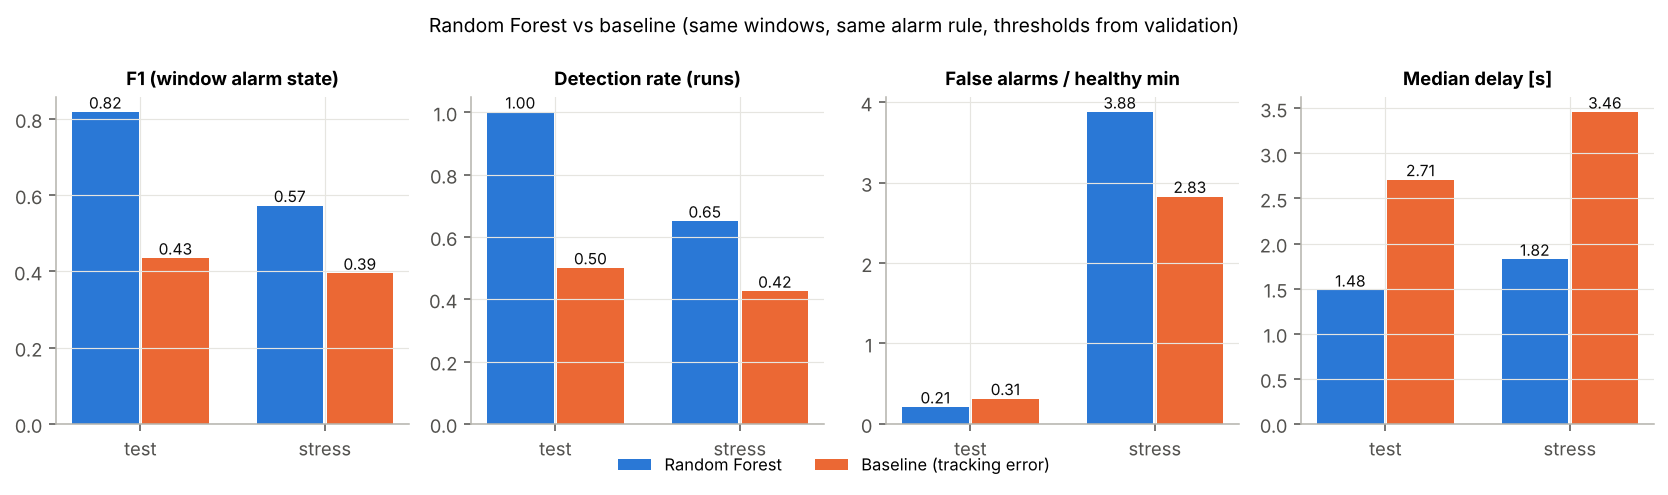
\includegraphics[width=.9\linewidth]{comparison_rf_vs_baseline.png}
\caption{Random Forest against the error-threshold baseline on the test and stress sets.}
\end{figure}

Inside the training range the Random Forest detected every faulty test run, while the baseline missed half, mostly mild
faults and faults on joint 1: with a threshold high enough to ignore fast healthy motion, error size alone misses
them. Maximum test delay was 11.2\,s, on a gradual fault. Window-level recall (0.69) is lower than the run-level
detection rate because windows inside the detection delay count as misses.

Outside the training range, the detector degrades sharply. Heavier loads and faster motion than it had seen were
read as friction: 15 of 20 healthy stress runs had at least one false alarm. On the sinusoidal stress runs, many
alarms were already on before the fault, so they could not count as detections. This is a direct negative answer to
the question's second half for conditions beyond the training range.

\begin{figure}[h]
\centering
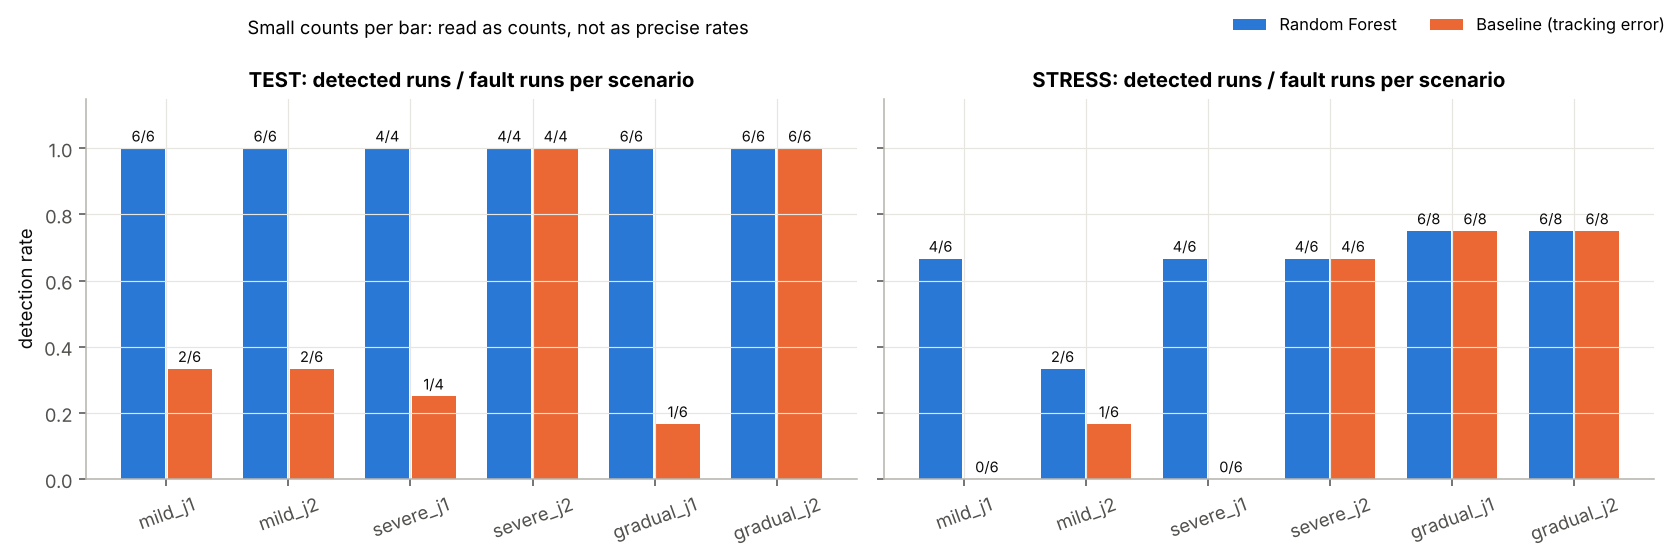
\includegraphics[width=.49\linewidth]{detection_by_scenario.png}\hfill
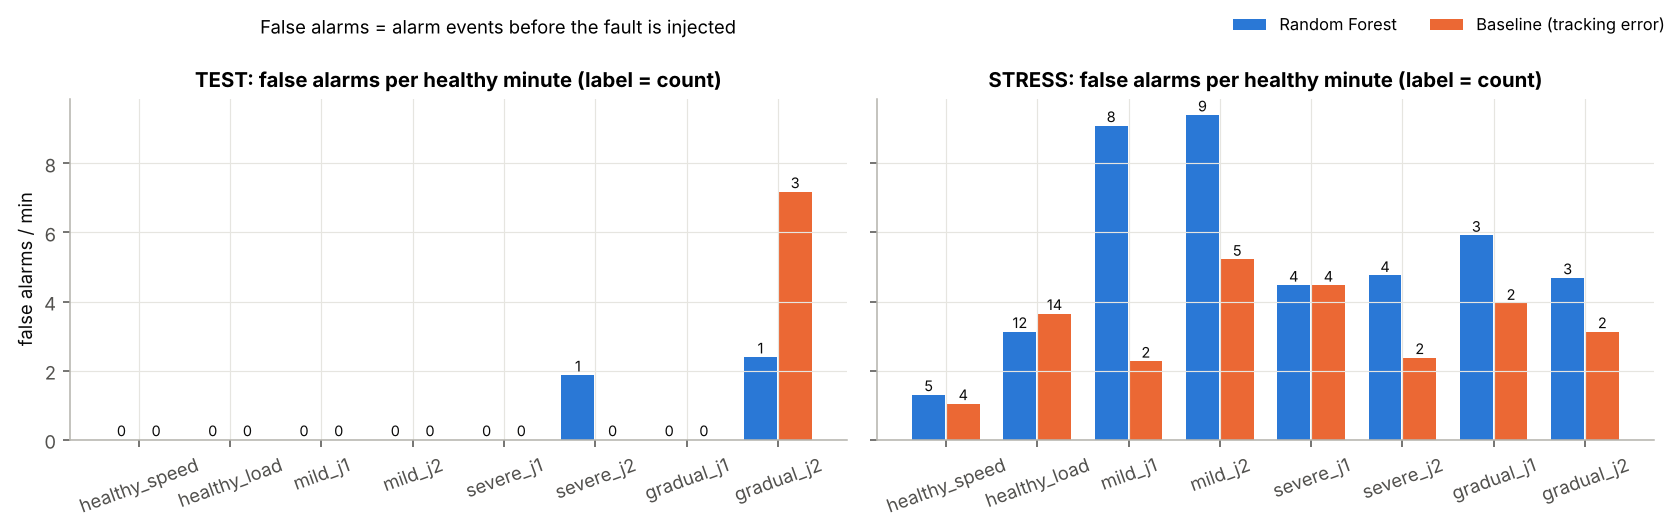
\includegraphics[width=.49\linewidth]{false_alarms_by_scenario.png}
\caption{Detections (left) and false alarms (right) per scenario.}
\end{figure}

\section{Diagnosis}
\subsection{Method}
An alarm alone (``check the joint'') does not tell a technician much. Once the alarm is on, a diagnosis stage reads
the same 24 features with two more Random Forests: a classifier for the faulty joint and a regressor for its friction
multiplier $m$. Both were trained only on anomalous, non-mixed training windows (13{,}027 windows, true $m$ from 1.62 to
4.00), with targets taken from ground truth. They reuse the detector's hyper-parameters and were not tuned. Online, the
per-window outputs are averaged over at most the last 20 above-threshold windows and shown only while the alarm is on,
for example \texttt{Joint 2 - friction increase: 213\% (x3.1)}. Test and stress data were first examined after this
stage was trained.

\subsection{Results}
\begin{table}[h]
\centering
\caption{Diagnosis on faulty runs that the detector caught. ``2\,s later'' includes only runs whose alarm was still
on and whose run had not ended.}
\begin{tabular}{llrrr}
\toprule
Set & When & Right joint & Median $|\hat m - m|$ & 90th pct.\ $|\hat m - m|$ \\
\midrule
Test   & alarm turns on & 30/32 & 0.36 & 0.68 \\
       & 2\,s later     & 23/23 & 0.20 & 0.64 \\
Stress & alarm turns on & 23/26 & 0.53 & 1.19 \\
       & 2\,s later     & 14/17 & 0.57 & 0.84 \\
\bottomrule
\end{tabular}
\end{table}

\begin{figure}[h]
\centering
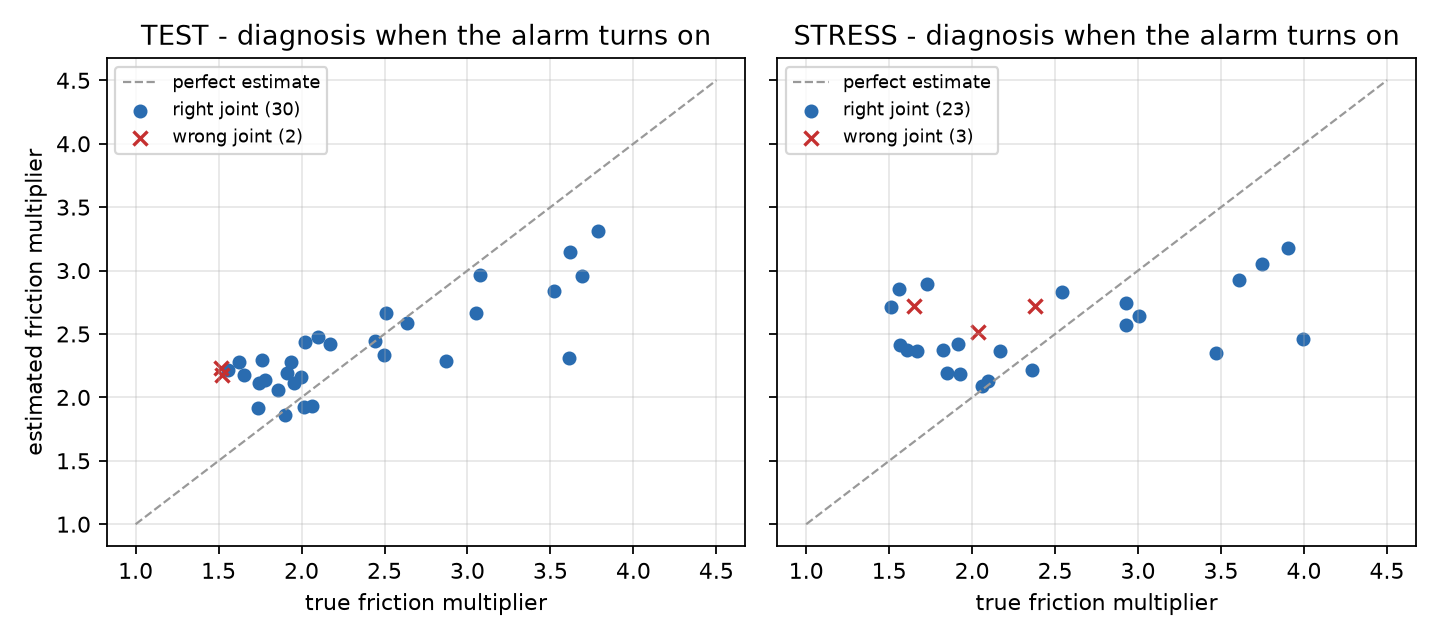
\includegraphics[width=\linewidth]{diagnosis_estimates.png}
\caption{Estimated against true friction multiplier at the moment the alarm turns on.}
\label{fig:diag}
\end{figure}

On the test set, both wrong joints came from gradual faults on joint 2 (runs R0225 and R0226), caught just as $m$
reached 1.51. Figure~\ref{fig:diag} shows a systematic pattern: estimates are pulled toward the middle of the training
range. Small increases near $m=1.5$ are overestimated at about 2.2, and large ones near 3.5--4 are underestimated. The
estimate is therefore good for telling a moderate fault from a severe one, but not for precise measurement. A median
error of 0.36 means, for example, reporting $+164\%$ when the truth is $+200\%$. Changes as small as the $\pm15\%$
healthy variation are below this resolution. On a false alarm the diagnosis still names a joint and a level, and both
are wrong; the diagnosis is only as trustworthy as the alarm before it.

\section{Limitations}
\begin{itemize}
  \item All data is simulated. The arm has rigid links and no motor, gearbox, backlash or temperature effects;
        simulated torque is not measured motor current.
  \item Only one fault type, on one joint at a time. The diagnosis gives a joint and a friction level, not a cause.
  \item The controller knows the exact nominal arm parameters; only the declared payload is slightly wrong.
  \item Test scenarios have 4--8 runs each, and no confidence intervals were computed.
  \item The models do not generalise to loads and speeds outside the training range.
  \item This is anomaly detection and diagnosis, not prediction of remaining useful life.
\end{itemize}

\section{Next steps}
\begin{itemize}
  \item Add physics-informed features, such as the residual between measured torque and the torque predicted by the
        nominal model, so that load and friction separate by construction; re-test on a fresh stress set, because the
        current one has already been examined.
  \item Detect out-of-range operating conditions and report ``uncertain'' instead of raising an alarm.
  \item Model motors and gearboxes, and compare with data from a real arm.
  \item Use run-to-failure data to study gradual degradation, the evidence needed for wear estimation.
  \item Add group-wise bootstrap confidence intervals and cross-validation.
\end{itemize}

\section{Reproducibility, materials and use of AI}
Seed 20261024; Python 3.13, NumPy 2.5.4, pandas 3.1.0, scikit-learn 1.9.1. The full pipeline, including the diagnosis
stage, runs with \texttt{python -m scripts.run\_pipeline --mode standard}; 31 automated tests cover physics, data
leakage, causality, online/offline consistency and the evaluation rules.

\begin{center}
\begin{tabularx}{.92\linewidth}{lX}
\toprule
Source code & \url{https://github.com/chechoutanh/JointGuard-AI} \\
Detailed results report & \href{https://github.com/chechoutanh/JointGuard-AI/blob/main/reports/standard/report_en.md}{\texttt{reports/standard/report\_en.md} on GitHub} \\
\bottomrule
\end{tabularx}
\end{center}

\noindent\textbf{Use of AI.} The code, experiments and reports were built with help from an AI coding assistant
(Claude), following my research question and decisions. I formulated the problem and the fault definition, specified
the simulation and evaluation design, ran the experiments and reviewed the results. Every number in this report is read
from the project's result files.

\end{document}
